\documentclass[pdf]{beamer}

\usepackage[utf8]{inputenc}
\usepackage[brazil]{babel}
\usepackage{graphicx}
\usepackage[normalem]{ulem}
\usepackage{listings}
\usepackage{hyperref}

\hypersetup{colorlinks=true,linkcolor=blue,urlcolor=blue,citecolor=blue,anchorcolor=blue}

\lstset{breakatwhitespace,
  language=C,
  columns=fullflexible,
  keepspaces,
  breaklines,
  tabsize=4,
  showstringspaces=false,
  extendedchars=true,
  keywordstyle=\color{blue}\ttfamily,
  stringstyle=\color{red}\ttfamily,
  commentstyle=\color{green!40!black}\ttfamily,
  morecomment=[l][\color{magenta}]{\#}
}

\lstset{breakatwhitespace,
  language=Python,
  columns=fullflexible,
  keepspaces,
  breaklines,
  tabsize=4,
  showstringspaces=false,
  extendedchars=true,
  keywordstyle=\color{blue}\ttfamily,
  stringstyle=\color{red}\ttfamily,
  commentstyle=\color{green!40!black}\ttfamily,
  morecomment=[l][\color{magenta}]{\#}
}

\usetheme{Warsaw}

\title[Outreachy]{Applying for Outreachy}

\author{{\Large Wander Lairson Costa}}
\institute{{\large Mozilla Corporation}}

\date{}

\begin{document}

\begin{frame}
  \titlepage
  \begin{center}
    \begin{tabular}{c l}
      \textbf{Email} & \href{mailto:wcosta@mozilla.com}{wcosta@mozilla.com} \\
      \textbf{Github} & \url{https://github.com/walac} \\
      \textbf{Twitter} & \href{https://twitter.com/walac00}{walac00} \\
    \end{tabular}
  \end{center}
\end{frame}

\begin{frame}{What is it?}
  \begin{itemize}
    \item A program for under represented groups
    \item It is not a quota system, it is an internship program
    \item \$5500 USD for 3 month remote internship
    \item \$500 USD for travel allowance
  \end{itemize}

  More info: \url{https://wiki.gnome.org/Outreachy}
\end{frame}

\begin{frame}{Eligible people}
  People who don't live in any of the following countries:
  \linebreak

  \begin{minipage}{.45\linewidth}
    \begin{itemize}
        \item Crimea
        \item Cuba
        \item Iran
    \end{itemize}
  \end{minipage}
  \hspace{.05\linewidth}
  \begin{minipage}{.45\linewidth}
    \begin{itemize}
        \item North Korea
        \item Syria
        \item Sudan
    \end{itemize}
  \end{minipage}

  \vspace{1em}
  And identify themselves as:
  \begin{itemize}
    \item Women (cis or trans)
    \item Trans men
    \item Genderqueers
    \item People of color living in USA
  \end{itemize}

  \begin{center}
    \begin{minipage}{.45\linewidth}
      \begin{itemize}
        \item Afro-american
        \item American indian
        \item Alaska Native
      \end{itemize}
    \end{minipage}
    \hspace{.05\linewidth}
    \begin{minipage}{.45\linewidth}
      \begin{itemize}
        \item Native Hawaiian
        \item Pacific Islander
        \item Hispanic/Latin
      \end{itemize}
    \end{minipage}
  \end{center}
\end{frame}

\begin{frame}{General steps}
  \textbf{You must have 40 hours/week available for internship}

  \begin{enumerate}
    \item Get in touch with mentor for the project you are applying for
    \item Join \texttt{\#outreachy} IRC channel at \url{irc.gnome.org}
    \item Make a contribution
    \item Apply at \url{https://outreachy.gnome.org}
  \end{enumerate}
\end{frame}

\begin{frame}{Mozilla specific}
  \begin{itemize}
    \item \texttt{\#outreachy} IRC channel at \url{irc.mozilla.org}
    \item Outreachy wiki page \url{https://wiki.mozilla.org/Outreachy}
    \item Interns join Mozilla All Hands
    \item Mentors receive orientation for mentorship
  \end{itemize}

  \begin{center}
    Larissa Shapiro \href{mailto:lshapiro@mozilla.com}{lshapiro@mozilla.com}\\
    Diversity and Inclusion Programs Manager
  \end{center}
\end{frame}

\begin{frame}{Tips}
  \begin{itemize}
    \item Talk to the project mentor either by IRC or email about first contribution
    \item Be honest about your skills and fears
    \item \textbf{Don't be afraid of asking questions}
    \item Don't pick the easiest task
    \item Apply early and apply for more than one project if you can
    \item Make more than one contribution if possible
    \item Use your social name when applying
    \item Contact former interns for orientation (they will get very happy to help)
    \item Familiarize yourself with IRC
  \end{itemize}
\end{frame}

\begin{frame}{Useful articles}
  \begin{itemize}
    \item \url{http://outreachy.anaplusplus.com/2016/05/what-is-outreachy-and-how-to-apply-for.html}
    \item \url{http://lwn.net/Articles/679038/}
    \item \url{https://vakila.github.io/blog/outreachy-what-how-why/}
  \end{itemize}
\end{frame}

\begin{frame}{FAQ}
  \begin{itemize}
    \item My english is bad.
    \item How to perform the first contact.
    \item I don't think I can make it.
    \item This project seems cool, but I have no idea where to start.
    \item I got a bug to work on, now I am completely lost.
    \item Mentor expectations.
  \end{itemize}
\end{frame}

\begin{frame}{Alternatives}
  \begin{itemize}
    \item University Internship
    \item Gsoc
    \item Job application
    \item Volunteer
  \end{itemize}
\end{frame}

\begin{frame}{Questions}
  \begin{center}
    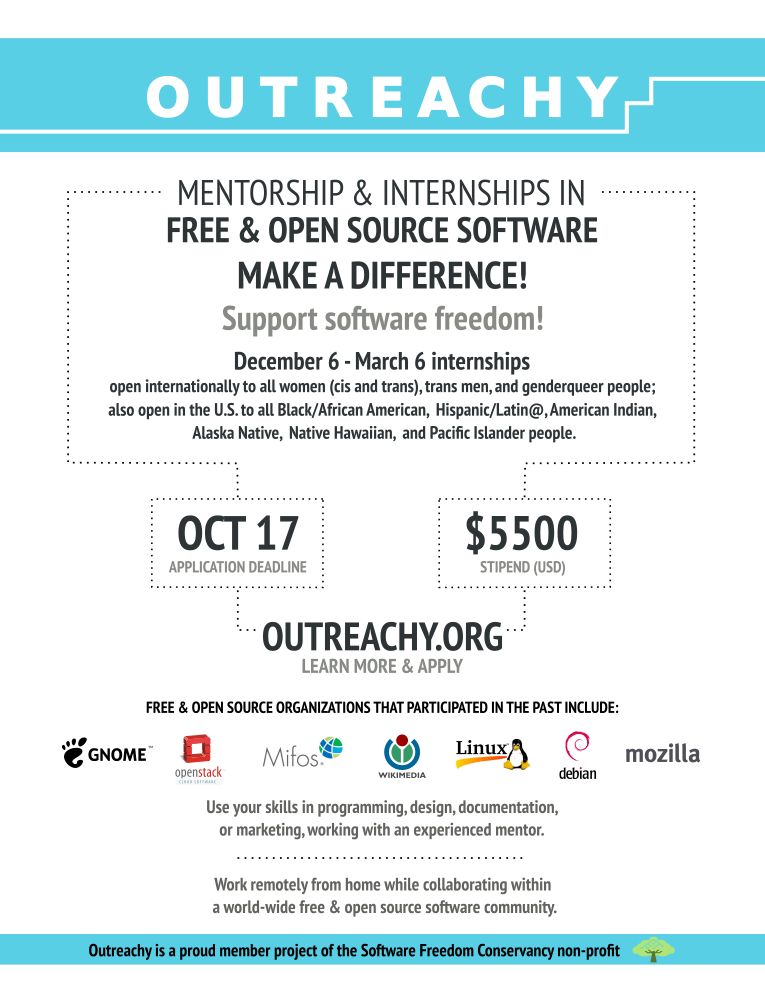
\includegraphics[scale=0.28]{img/outreachy-applicants-2016-December.png}
  \end{center}
\end{frame}

\end{document}

